\documentclass{report}
\usepackage[utf8]{inputenc}
\usepackage[top=0cm, bottom=0cm, left=2cm, right=2cm]{geometry}
\usepackage[francais]{babel}
\usepackage[T1]{fontenc}
\usepackage{graphicx}
\usepackage{subcaption}


\begin{document}


\chapter{entreprise} 
	\section{biomedia (Imperial college, department of computing (biomedical image analysis section) )}

	La mission du groupe BioMedIA est de développer de nouvelles techniques de
	calcul pour l'analyse d'images biomédicales. Le groupe se concentre sur des
	domaines de recherche de pointe, y compris:

	- Le développement d'algorithmes d'acquisition, d'analyse et d'interprétation
	des images. En particulier dans les domaines du recalage, de la reconstruction,
	du suivi de mouvement, de la segmentation et de la modélisation.

	- L'apprentissage machine pour l'extraction d'information clinique à partir
	d'images médicales. Les applications incluent le diagnostic assisté par
	ordinateur, la planification automatisée de traitement médicale, ou encore les
	interventions et la thérapie guidées par ordinateur.

	Nous nous intéressons particulièrement à l'imagerie et les technologies de
	traitement informatique qui nous permettent de mieux comprendre le
	développement du cerveau humain, l’évolution des maladies mentales et le
	diagnostic des patients atteints de maladie cardiovasculaire.

	\section{MIRTK}
	 => stable mais nécessite une maintenance et une amélioration continue pour rester pertinent.
	 Intervention sur le module "Numerics", bibliotèque mathématique.
\chapter{ objectifs/cahiers des charges}
	\section{problématique (+contexte)}
	Arrayfire:Bibliothèque mathématique fournissant plusieurs fonctions de manipulation de matrices, ainsi que la possibilité de faire des boucles parallèles
	- Simplifier le code - Optimiser les performances de calcul -
	\section{cahier des charges}
	- Intégrer ArrayFire à MIRTK, aussi bien au niveau des manipulations mathématiques qu'à celui de la programmation parallèle.
	\newline- Enlever toute dépendance de MIRTK à TBB
	\newline- Le délivrable sera composé de 2 backends, l'un AF et l'autre EIGEN. En fonction des applications, un switch automatique entre chaque structure sera appelé en dur grâce à des commandes pré-proc.
	\newline- La programmation sera réalisée de manière transparente, c'est-à-dire que MIRTK doit réaliser les mêmes fonctions et garder la même API même si le code plus en profondeur est modifié.
	\newline- Plusieurs benchmarks affirmeront les performances d'ArrayFire et de l'optimisation globale de MIRTK.
	\section{objectifs et milestones}
	\subsection{Objectifs}- Ajouter ArrayFire à MIRTK, en remplaçant les fonctions d'EIGEN les moins adaptées par les fonctions d'AF
	- Faire un profiling des fonctions concernées par TBB, et interpréter les résultats afin d'élaborer une stratégie pour implanter la programmation // d'AF.
	- Supprimer er les TBB inutiles ou peu efficaces, et remplacer les autres par l'équivalent d'AF (gfor).
	- 
	
	\subsection{Diagramme de GANTT}
	 => gantt chart prévisionnel
	\begin{figure}[h!]
		\begin{center}
			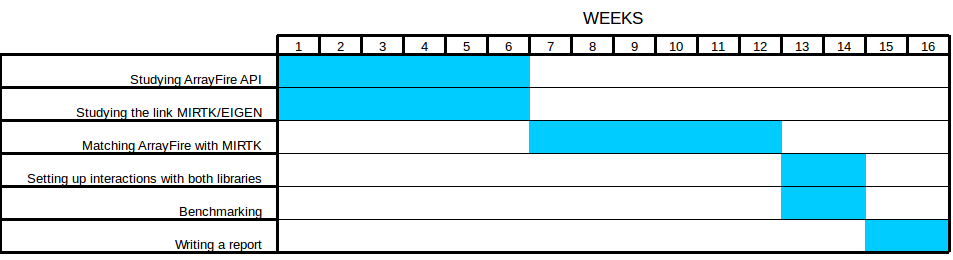
\includegraphics[width=18cm]{Reports/figures/estimated_gantt.png}
		\end{center}	
		\caption{Diagramme de GANTT prévisionnel}
		\label{Diagramme de GANTT prévisionnel}
	\end{figure}
\chapter{ réalisation}
	\section{profiling}
	Profiling => on identifie les fonctions sur lesquelles agir en premier
	On utilise Valgrind, qui, avec callgrind analyse la manière dont les caches sont utilisés, puis on double check avec VTune sur une autre machine.
	\section{integration d'arrayfire dans MIRTK}
	\section{benchmarking}
	 
	
\end{document}
